% ============================================================
% KAPITEL 4 — KONZEPT
% ============================================================

\chapter{Konzept}
\label{ch:konzept}

Dieses Kapitel entwickelt aus den Anforderungen das Lösungskonzept.
Nach einem Überblick beschreibt es den Entwurfsraum der drei Repräsentationsformen, die Entwurfsentscheidungen für einen fairen Vergleich, die Idee zur Steuerung der hybriden Form und die Begründung dafür, den Erfolg nach Referenztypen getrennt zu betrachten.
Die technische Umsetzung folgt in Kapitel~\ref{ch:implementierung}.


% ------------------------------------------------------------
\section{Lösungsansatz im Überblick}
\label{sec:konz-ueberblick}

Der Lösungsansatz beruht auf einem sprachgesteuerten Agenten.
Er nimmt einen natürlichsprachlichen Befehl entgegen, verschafft sich über eine Repräsentation ein Bild der Szene und verändert sie über eine feste Menge von Operationen.
Der entscheidende Freiheitsgrad des Entwurfs ist die Form, in der dem Agenten die Szene bereitgestellt wird, und diese Form ist zugleich der Untersuchungsgegenstand.

Die Arbeit geht in drei Schritten vor.
Zuerst werden verschiedene Repräsentationsformen unter gleichen Bedingungen verglichen, um ihren Einfluss zu bestimmen (RQ1).
Danach wird untersucht, ob sich die Kombination der Repräsentationen gezielt verbessern lässt (RQ2).
Zuletzt wird die beste Variante in die immersive Zielumgebung übertragen und dort als Demonstrator erprobt, um die Übertragbarkeit zu zeigen.


% ------------------------------------------------------------
\section{Repräsentationsformen}
\label{sec:konz-repraesentationen}

Der Entwurfsraum umfasst drei Formen, in denen die Szene dem Agenten bereitgestellt werden kann.

Die strukturelle Form beschreibt die Szene als exakte Daten.
Sie kennt die Objekte mit Kennungen, Typen, Positionen und Größen und ist damit stark bei allem, was sich aus diesen Daten ableiten lässt, etwa bei geometrischen Beziehungen.
Was in den Daten nicht kodiert ist, bleibt ihr verborgen.

Die visuelle Form beschreibt die Szene über eine gerenderte Ansicht, die ein visuelles Modell interpretiert.
Sie erfasst das Aussehen der Szene und ist damit stark bei Eigenschaften, die nur im Bild erkennbar sind, liefert aber keine exakten Koordinaten.
Wie in Abschnitt~\ref{sec:grundlagen-modelle} beschrieben, erreicht sie das entscheidende Sprachmodell nur als sprachliche Beschreibung, die das Sprach-Bild-Modell aus dem Bild erzeugt.

Die hybride Form stellt beide Schichten zugleich bereit und erlaubt damit, exakte Geometrie und Aussehen gemeinsam zu berücksichtigen.
Im Kontext des Sprachmodells treffen in ihr eine exakte, aber unvollständige Datenstruktur und eine reichhaltige, aber unscharfe Beschreibung aufeinander.

Mit diesen drei Formen sind die beiden Einzelquellen und ihre Kombination abgedeckt.
Der Vergleich der Einzelformen zeigt, wofür jede Schicht zuständig ist, der Vergleich mit der hybriden Form, ob eine Kombination die Stärken beider vereint.

Bewusst festgelegt ist der Inhalt der strukturellen Schicht.
Sie enthält je Objekt Kennung, Typ, Position, Farbe und Größe sowie die Pose der Kamera, aber keine vorberechneten räumlichen Beziehungen.
Eine Relation wie \enquote{links von} muss der Agent selbst aus den Koordinaten ableiten.
Andernfalls würde die Auswertung die Güte einer Vorverarbeitung messen und nicht die Eignung der Repräsentation.


% ------------------------------------------------------------
\section[Entwurfsentscheidungen]{Entwurfsentscheidungen für einen fairen Vergleich}
\label{sec:konz-fairness}

Damit der Vergleich die Repräsentation misst und nicht einen Nebeneffekt des Aufbaus, darf keine Variante aus Gründen bevorzugt oder benachteiligt werden, die mit ihrer Repräsentation nichts zu tun haben.
Drei Entwurfsentscheidungen dienen diesem Zweck.

Alle Varianten sprechen Objekte über dieselben Kennungen an.
Eine Kennung ist dabei nur ein Adressierungsmittel und kein Bestandteil des Szenenverständnisses.
Die visuelle Variante wird über Marken, die in das gerenderte Bild eingezeichnet werden, an dieselben Kennungen gebunden, nach dem Set-of-Mark-Prinzip~\cite{yang2023}.
So kann auch sie ein erkanntes Objekt benennen, ohne dadurch einen strukturellen Vorteil zu erhalten.

Für Bewegungen stellt das System neben einer absoluten auch eine relative Operation bereit, mit der sich Objekte ohne exakten Weltbezug verschieben lassen.
Fehlte sie, wäre die visuelle Variante benachteiligt, weil sie keine exakten Koordinaten kennt, und dieser Nachteil ginge auf den Zuschnitt der Werkzeuge zurück, nicht auf die Repräsentation.

Schließlich wird Information gezielt weggelassen.
Die unterscheidende Eigenschaft der rein perzeptuellen Aufgaben, etwa ein Oberflächenmuster, wird absichtlich nicht in die strukturelle Schicht aufgenommen.
Nur so entsteht ein Fall, in dem die strukturelle Schicht prinzipiell blind ist und die exklusive Kompetenz der visuellen Schicht sichtbar werden kann.


% ------------------------------------------------------------
\section{Steuerung der Modalitätsfusion}
\label{sec:konz-fusion}

Die hybride Form stellt beide Schichten bereit, legt aber nicht fest, wie der Agent sie gegeneinander gewichtet.
Das Konzept geht davon aus, dass die bloße Verfügbarkeit beider Schichten nicht ausreicht, damit ihre Stärken auch zusammenwirken.
Gestützt wird diese Annahme durch eine Analogie zu Beobachtungen, nach denen multimodale Modelle bei widersprüchlichen Eingaben der textuellen Information den Vorrang geben~\cite{deng2025, wu2025}.
Da hier keine Bild- und Textquelle, sondern zwei Textquellen konkurrieren (Abschnitt~\ref{sec:grundlagen-sota}), lautet die Erwartung genauer, dass die exaktere Quelle die unschärfere überschreibt, auch wo nur die unschärfere die Antwort enthält.
Wie die beiden Schichten dem Agenten präsentiert werden, wird damit selbst zum Entwurfsgegenstand.

Das Konzept sieht dafür zwei Strategien vor.
Bei der Priorisierung wird eine der beiden Schichten für einen bestimmten Zweck für maßgeblich erklärt und in den Vordergrund gestellt.
Bei der Kompetenztrennung erhalten die beiden Schichten getrennte Zuständigkeiten, sodass jede nur für den Teil der Aufgabe herangezogen wird, für den sie geeignet ist.

Beide Strategien wirken ausschließlich über die Instruktion; die Modelle werden nicht nachtrainiert, ihre Gewichte bleiben unverändert.
Diese Beschränkung ist gewollt.
Sie hält den Vergleich sauber, weil sich nur der Kontext ändert, und sie passt zur Fragestellung, die nach der Repräsentation und nicht nach einer Modellanpassung fragt.
Wie die beiden Strategien konkret formuliert sind, beschreibt Kapitel~\ref{ch:implementierung}.


% ------------------------------------------------------------
\section{Differenzierung nach Referenztyp}
\label{sec:konz-referenztyp}

Ob eine Repräsentation eine Aufgabe lösen kann, hängt davon ab, wie der Befehl auf ein Objekt verweist.
Ein Verweis über eine exakte Lage stellt andere Anforderungen als einer über eine sichtbare Eigenschaft.
Die beiden Repräsentationen sind daher nicht nur unterschiedlich stark, sondern teilweise für einander ausschließende Bereiche zuständig, und dieser Gedanke trägt das gesamte Konzept.

Manche Referenzen lassen sich nur über die strukturelle Schicht auflösen: Ein Objekt, das im Bild verdeckt ist, bleibt in den strukturellen Daten verzeichnet.
Andere lassen sich nur über die visuelle Schicht auflösen: Ein Oberflächenmuster, das in den strukturellen Daten nicht vorkommt, ist nur im Bild erkennbar.
Dazwischen liegt ein Bereich, in dem beide Schichten dieselbe Referenz auflösen können.

Abbildung~\ref{fig:venn} stellt diese Verteilung dar.
Die einander ausschließenden Bereiche sind der Grund, warum eine Kombination beider Schichten überhaupt sinnvoll ist, und zugleich der Grund, den Erfolg nach Referenztypen aufzuschlüsseln statt als einen einzelnen Gesamtwert zu berichten.
Die konkrete Einteilung der Referenztypen und die zugehörigen Szenarien führt Kapitel~\ref{ch:evaluation} ein.

\begin{figure}[htbp]
  \centering
  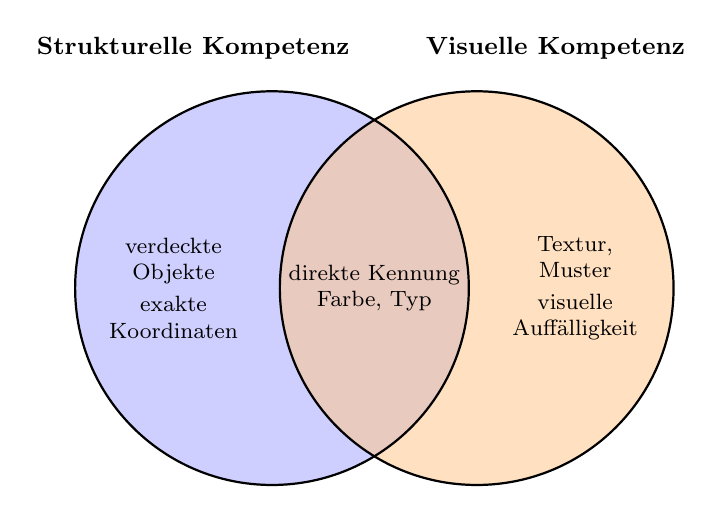
\begin{tikzpicture}[font=\small]
    \begin{scope}[fill opacity=0.55]
      \fill[blue!35]   (-1.3,0) circle (2.5);
      \fill[orange!45] ( 1.3,0) circle (2.5);
    \end{scope}
    \draw[thick] (-1.3,0) circle (2.5);
    \draw[thick] ( 1.3,0) circle (2.5);
    \node[font=\small\bfseries] at (-2.3,3.05) {Strukturelle Kompetenz};
    \node[font=\small\bfseries] at ( 2.3,3.05) {Visuelle Kompetenz};
    \node[align=center, font=\footnotesize] at (-2.55,0)
      {verdeckte\\Objekte\\[2pt]exakte\\Koordinaten};
    \node[align=center, font=\footnotesize] at (0,0)
      {direkte Kennung\\Farbe, Typ};
    \node[align=center, font=\footnotesize] at (2.55,0)
      {Textur,\\Muster\\[2pt]visuelle\\Auffälligkeit};
  \end{tikzpicture}
  \caption{Konzeptionelle Kompetenzverteilung der beiden Repräsentationen. Der Überlappungsbereich steht für Referenzen, die beide Schichten auflösen können, die Außenbereiche für die exklusive Kompetenz jeweils einer Schicht. Aus diesen exklusiven Bereichen ergibt sich der Nutzen des hybriden Ansatzes.}
  \label{fig:venn}
\end{figure}
